% !TEX root = main.tex

\section{图像复原}
图像增强是主观的,图像复原则是客观的(恢复原图)。

空间域和频率域的退化图像分别可以由下式的退化模型给出
\[\begin{aligned}
g(x,y)&=h(x,y)*f(x,y)+\eta(x,y)\\
G(u,v)&=H(u,v)F(u,v)+N(u,v)
\end{aligned}\]
关键在于怎么找回$f$和$F$,而$h$属于系统噪声。

\begin{figure}[H]
\centering
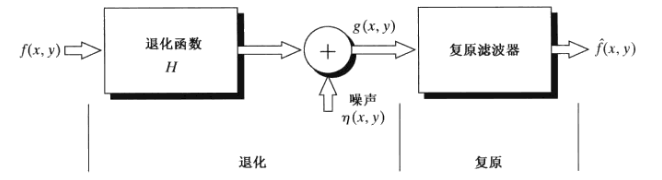
\includegraphics[width=0.8\linewidth]{fig/restoration.png}
\end{figure}

\subsection{噪声模型}
\begin{itemize}
\item 高斯噪声
\[p(z)=\frac{1}{\sqrt{2\pi}\sigma}\ee^{-\frac{(z-\bar{z})^2}{2\sigma^2}}\]
\item 脉冲/椒盐噪声
\[p(z)=\begin{cases}
P_a & z=a\\
P_b & z=b\\
1-P_a-P_b & \text{others}
\end{cases}\]
\item 瑞利噪声:均值$\bar{z}=a+\sqrt{\pi b/4}$,方差$\sigma^2=b(4-\pi)/4$
\[p(z)=\begin{cases}
\frac{2}{b}(z-a)\ee^{-(z-a)^2}{b} & z\geq a\\
0 & z<a
\end{cases}\]
\item 爱尔兰/伽马噪声:均值$\bar{z}=b/a$,方差$\sigma^2=b/a^2$
\[p(z)=\begin{cases}
\frac{a^bz^{b-1}}{(b-1)!}\ee^{-az} & z\geq a\\
0 & z<a
\end{cases},\;a>0,b\in\zz^+\]
\item 指数噪声:均值$\bar{z}=1/a$,方差$\sigma^2=1/a^2$
\[p(z)=\begin{cases}
a\ee^{-az} & z\geq 0\\
0 & z<0
\end{cases}\]
\item 均匀噪声:均值$\bar{z}=(a+b)/2$,方差$\sigma^2=(b-a)^2/12$
\[p(z)=\begin{cases}
\frac{1}{b-a} & a\leq z\leq b\\
0 & \text{others}
\end{cases}\]
\end{itemize}
\begin{figure}[H]
\centering
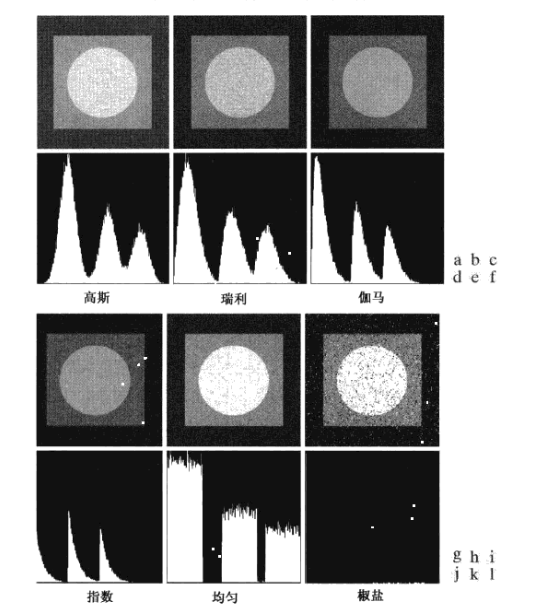
\includegraphics[width=0.5\linewidth]{fig/noise.png}
\end{figure}

\subsection{噪声存在下的空间滤波复原}
考虑唯一存在噪声退化,即不存在系统退化,则原式变为
\[\begin{aligned}
g(x,y)&=f(x,y)+\eta(x,y)\\
G(u,v)&=F(u,v)+N(u,v)
\end{aligned}\]

\subsubsection{均值滤波器}
\begin{itemize}
	\item 算术均值滤波
	\[\hat{f}(x,y)=\frac{1}{MN}\sum_{(s,t)\in S_{xy}}g(s,t)\]
	\item 几何均值滤波
	\[\hat{f}(x,y)=\lrs{\prod_{(s,t)\in S_{xy}}g(s,t)}^{\frac{1}{mn}}\]
	相比算术均值,丢失图像细节比较少
	\item 谐波均值滤波
	\[\hat{f}(x,y)=\frac{mn}{\sum_{(s,t)\in S_{xy}}\frac{1}{g(s,t)}}\]
	对盐(大的)噪声比较好,对胡椒噪声不好,善于处理高斯噪声
	\item 逆谐波均值滤波
	\[\hat{f}(x,y)=\frac{\sum_{(s,t)\in S_{xy}}g(s,t)^{Q+1}}{\sum_{(s,t)\in S_{xy}}g(s,t)^Q}\]
	其中$Q$称为滤波器的阶数,适合减少椒盐噪声的影响。
	当$Q$为正时,消除胡椒噪声;当$Q$为负时,消除盐粒噪声;但不能同时消除这两种噪声。
	当$Q=0$时退化为算术均值,$Q=-1$为谐波均值滤波
\end{itemize}

\subsubsection{状态/顺序统计滤波器}
\begin{itemize}
	\item 最大滤波器
	\item 最小滤波器
	\item \textbf{中点}滤波器:
	\[\hat{f}(x,y)=\frac{1}{2}[\max_{(x,y)\in S_{xy}}g(s,t)+\min_{(x,y)\in S_{xy}}g(s,t)]\]
	\item 修正阿尔法均值滤波器:去除$d/2$个最大值(去盐)和$d/2$最小值(去椒),再取平均(去高斯)
	\[\hat{f}(x,y)=\frac{1}{mn-d}\sum_{(x,y)\in S_{xy}}g_r(s,t)\]
\end{itemize}

\subsubsection{自适应滤波器}
滤波器作用于局部区域$S_{xy}$,$\sigma^2_\eta$为干扰$f(x,y)$以形成$g(x,y)$的噪声方差,$m_L$为局部均值,$\sigma_L^2$为局部方差
\[\hat{f}(x,y)=g(x,y)-\frac{\sigma^2_\eta}{\sigma^2_L}[g(x,y)-m_L]\]
满足以下假设
\begin{itemize}
	\item 如果$\sigma_\eta^2$为$0$,则应直接返回$g(x,y)$的值
	\item 如果局部方差与$\sigma_\eta^2$高度相关,则滤波器返回$g(x,y)$的近似值。
	典型地,高局部方差与边缘相关,应该保护这些边缘
	\item 如果两个方差相等,则希望滤波器返回$S_{xy}$中像素的算术均值。这种情况发生在局部区域与整个图像有相同特性地条件下,局部噪声将通过简单地求平均来降低。
\end{itemize}

\subsection{通过频域滤波抑制噪声}
\subsubsection{带阻滤波器}
只有中间$W$宽度的能够通过,同样有理想带阻滤波器、布特沃斯滤波器、高斯带阻滤波器
\[H(u,v)=\begin{cases}
1 & D(u,v)<D_0-\frac{W}{2}\lor D(u,v)>D_0+\frac{W}{2}\\
0 & \text{otherwise}
\end{cases}\]
带阻滤波可以消除周期性噪声。
\begin{figure}[H]
\centering
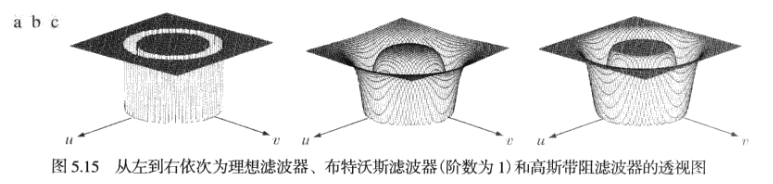
\includegraphics[width=0.8\linewidth]{fig/BSF.png}
\end{figure}

\subsubsection{带通滤波器}
\[H_{bp}(u,v)=1-H_{br}(u,v)\]
只是将带阻滤波器取反

\subsubsection{陷波滤波器}
阻止(或通过)事先定义得中心频率邻域内的频率
\begin{figure}[H]
\centering
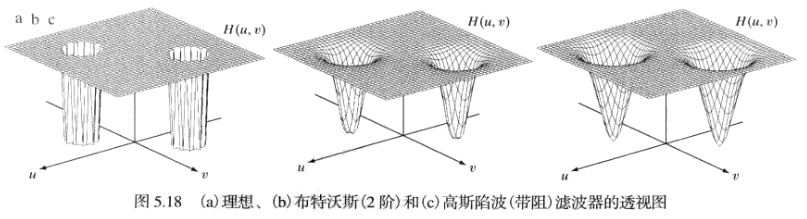
\includegraphics[width=0.8\linewidth]{fig/notch.png}
\end{figure}

由于频率域的共轭对称性,去掉一个,要去除另一个对称的频率。

陷波带通滤波器可以用于确定噪声模式。

如何评判图像的好坏
\begin{itemize}
\item 方差最小,噪声水平最低
\item 是不是平滑的
\end{itemize}

\subsection{线性、位置不变的退化}
输入/输出关系可以表示为
\[g(x,y)=H[f(x,y)]+\eta(x,y)\]

具有加性噪声的线性空间不变退化系统,可在空间域建模为退化(点扩散)函数与一幅图像的卷积,然后再加上噪声。
基于卷积定理,在频率域中,同样的过程可表示为图像和退化函数的变换的乘积,然后再加上噪声的变换。

\subsection{估计退化函数}
\begin{itemize}
	\item 观察法
	\[H_s(u,v)=\frac{G_s(u,v)}{\hat{F}_s(u,v)}\]
	\item 实验法:获取与退化图像类似的装置,由成像一个亮点得到退化的冲激响应
	\[A\delta(x,y)\to g(x,y)\iff A\to G(u,v)\]
	故$H(u,v)=\frac{G(u,v)}{A}$
	\item 数学建模法:如运动模糊
	\[g(x,y)=\intabu{0}{T}{f[x-x_0(t),y-y_0(t)]}{t}\]
	最终得到退化函数
	\[H(u,v)=\intabu{0}{T}{\ee^{-j2\pi[ux_0(t)+vy_0(t)]}}\]
\end{itemize}

\subsection{逆滤波}
对于线性移不变系统的退化模型为
\[G(u,v)=H(u,v)F(u,v)+N(u,v)\]
如果知道$H(u,v)$,则可以计算原始图像的傅里叶变换估计(去卷积)
\[\hat{F}(u,v)=\frac{G(u,v)}{H(u,v)}=F(u,v)+\frac{N(u,v)}{H(u,v)}\]
如果$H(u,v)$很小,则$N(u,v)/H(u,v)$将很大,估计就会失败。

维纳滤波:最佳去噪滤波器
\[\hat{F}(u,v)=\frac{P_f(u,v)}{P_f(u,v)+P_k(u,v)}=\frac{P_f(u,v)}{P_f(u,v)+\lrabs{\frac{N(u,v)}{H(u,v)}}}\]